\documentclass[aspectratio=169,11pt]{beamer}
\usepackage{presentation-theme}
\hypersetup{pdftitle={Diffusion encoder: token chemistry and sparse features},pdfauthor={Wuhao},pdfsubject={Pinned native JAX diffusion checkpoint comparison, 30 September 2026}}
\newcommand{\bodytext}[4]{\node[anchor=north west,inner sep=0,align=left,text width=#3cm,font=\figurefont\fontsize{10}{13}\selectfont] at (#1,#2) {#4};}
\newcommand{\plotfigure}[1]{\node[anchor=north,inner sep=0] at (8,6.78) {\includegraphics[width=14.3cm,height=4.75cm,keepaspectratio]{figures/#1_slide.pdf}};}
% Generated only from completed, verified artifacts. The build refuses missing results.
% Generated from completed artifacts by prepare_results.py.
\newcommand{\DiffusionVerdict}{Diffusion scores lower than both JEPA checkpoints on the shared final-token chemical readout.}
\newcommand{\DiffusionPrimaryNumber}{0.7244}
\newcommand{\DiffusionTakeaway}{A matched token-level evaluation; training exposure and native input quantization still differ.}
\newcommand{\ReadoutTitle}{Diffusion trails the final-token chemical readout}
\newcommand{\ReadoutTakeaway}{Diffusion attention gains +0.0016 MACCS AUROC over mean; its paired interval includes zero.}
\newcommand{\MaccsTargetCount}{145}
\newcommand{\FunctionalTargetCount}{13}
\newcommand{\BootstrapCount}{1,000}
\newcommand{\BootstrapDefined}{980}
\newcommand{\PairedTitle}{Paired molecules separate the checkpoint differences}
\newcommand{\PairedTakeaway}{Attention differences: parent -0.0744; periodic -0.0506 MACCS AUROC.}
\newcommand{\SaeTitle}{Sparse reconstruction and chemical recognition are separate}
\newcommand{\SaeTakeaway}{Diffusion k=32 seed0: 92.8\% held-out variance explained; 3 chemical candidates frozen before test.}
\newcommand{\ChemicalCandidateSummary}{The strongest hydroxyl candidate (f4682) has test AUROC 0.744, but also mass correlation 0.599; strict matched-pair ordering is 0.517.}
\newcommand{\RelativeLTwoNote}{original-unit relative L2 is 0.259 for diffusion versus 0.088 / 0.054 for parent / periodic.}
\newcommand{\ClosingTakeaway}{Token-level readouts answer chemical accessibility; SAE structure adds a separate, qualified view.}

\begin{document}

% 1: Scope, verified checkpoint identity, and the actual measured conclusion.
\begin{frame}
\begin{tikzpicture}[remember picture,overlay,shift={(current page.south west)}]
\header{DIFFUSION ENCODER / 30 SEP 2026}{}
\node[anchor=north west,inner sep=0,font=\brandmedium\fontsize{25}{29}\selectfont,text width=13.8cm,align=left] at (.75,7.25) {How do diffusion-trained\\tokens compare chemically?};
\bodytext{.85}{5.10}{13.8}{\DiffusionVerdict}
\node[anchor=north west,inner sep=0,font=\brandmedium\fontsize{29}{33}\selectfont] at (.85,3.45) {\DiffusionPrimaryNumber};
\bodytext{.85}{2.42}{13.8}{Final-token attention MACCS AUROC; diffusion checkpoint 831,000}
\takeaway{\DiffusionTakeaway}
\source{Latest committed endpoint of adiff-1p8b-ep-v6e32-4d-20260922-080322, pinned by 60 object generations. Comparison arms: frozen-teacher JEPA 1,190k and periodic-teacher JEPA 1,209k.}
\end{tikzpicture}
\end{frame}

% 2: A token-preserving protocol; sparse decomposition is a separate endpoint.
\begin{frame}
\begin{tikzpicture}[remember picture,overlay,shift={(current page.south west)}]
\header{01 / SHARED EVALUATION}{Preserve peak tokens for chemical readouts and sparse analysis}
\plotfigure{native_token_sae}
\takeaway{Token attention is the primary chemistry endpoint; sparse reconstruction measures a different property.}
\source{One representative spectrum per molecular connectivity: 4,096 train / 1,024 validation / 1,024 test. Native JAX BF16, batch 8; physical peaks exclude CLS and padding. Exact native/instrumented/cache parity required.}
\end{tikzpicture}
\end{frame}

% 3: Complete numbers and intervals are generated from the new analyzer.
\begin{frame}
\begin{tikzpicture}[remember picture,overlay,shift={(current page.south west)}]
\header{02 / TOKEN-AWARE CHEMISTRY}{\ReadoutTitle}
\plotfigure{final_token_auroc}
\takeaway{\ReadoutTakeaway}
\source{Final state 27; matched physical-token mean control and learned attention. AUROC of mean logits across three independently fitted seeds. Shared fixed support: \MaccsTargetCount\ MACCS / \FunctionalTargetCount\ functional-group targets; 1,024 test molecules.}
\end{tikzpicture}
\end{frame}

% 4: Report paired molecule uncertainty, not an independent-error comparison.
\begin{frame}
\begin{tikzpicture}[remember picture,overlay,shift={(current page.south west)}]
\header{03 / PAIRED CHECKPOINT DIFFERENCES}{\PairedTitle}
\plotfigure{paired_readout_differences}
\takeaway{\PairedTakeaway}
\source{Diffusion minus comparison; positive favors diffusion. Shared molecule-bootstrap counts; \BootstrapDefined\ of \BootstrapCount\ MACCS resamples retain both classes for every fixed target. Undefined replicates omitted. Descriptive 95\% intervals; no pretraining-seed uncertainty or multiplicity correction.}
\end{tikzpicture}
\end{frame}

% 5: Do not equate sparse reconstruction with semantic alignment.
\begin{frame}
\begin{tikzpicture}[remember picture,overlay,shift={(current page.south west)}]
\header{04 / SPARSE TOKEN FEATURES}{\SaeTitle}
\plotfigure{sae_quality_and_associations}
\takeaway{\SaeTakeaway}
\source{Raw19, 8,192 features; train-only normalization and equal molecule weights. FVE is relative to the training mean; \RelativeLTwoNote\ Right: all frozen candidates per concept, paired molecule 95\% intervals; missing candidates remain gaps. No diffusion feature interventions.}
\end{tikzpicture}
\end{frame}

% 6: The run identifiers do not imply weight continuation.
\begin{frame}
\begin{tikzpicture}[remember picture,overlay,shift={(current page.south west)}]
\header{05 / WHAT THIS COMPARISON IDENTIFIES}{Shared dataset, distinct training histories and native inputs}
\node[anchor=north west,inner sep=0,font=\brandmedium\fontsize{15}{18}\selectfont] at (1.0,6.50) {Training exposure};
\bodytext{1.0}{5.62}{6.1}{All three logs begin at step 0.\\Nominal spectrum presentations:\\Parent: 1.219 billion\\Periodic: 1.238 billion\\Diffusion: 0.851 billion}
\draw[line] (7.7,2.40)--(7.7,6.55);
\node[anchor=north west,inner sep=0,font=\brandmedium\fontsize{15}{18}\selectfont] at (8.25,6.50) {Native input difference};
\bodytext{8.25}{5.62}{6.05}{Diffusion quantizes $m/z$ into\\0.48828125-Da bin midpoints\\before Fourier embedding.\\\vspace{3mm}JEPA arms retain continuous $m/z$.\\The loss alone is not isolated.}
\takeaway{Compare the measured endpoints; do not attribute the difference solely to the diffusion objective.}
\source{Pinned checkpoint contracts share dataset revision, manifest and shard-plan hashes. Nominal presentations = global step $\times$ configured global batch 1,024, not unique spectra; accumulation is already included. Teacher histories are not added.}
\end{tikzpicture}
\end{frame}

% 7: Reproduction and strict claim boundaries.
\begin{frame}
\begin{tikzpicture}[remember picture,overlay,shift={(current page.south west)}]
\header{06 / EVIDENCE AND REPRODUCTION}{A bounded checkpoint comparison, with reusable artifacts}
\bodytext{1.0}{6.55}{13.6}{\textbf{Checkpoint provenance}\\Run config, latest committed object generations, CRC32C and lineage evidence; no parent initialization is specified for diffusion.}
\bodytext{1.0}{5.04}{13.6}{\textbf{Chemical features need nuisance controls}\\\ChemicalCandidateSummary}
\bodytext{1.0}{3.50}{13.6}{\textbf{Claim boundaries}\\No matched training-budget experiment, pretraining-seed replication, diffusion feature ablation or validated peak-to-fragment assignments. Readout scores are not calibrated chemical probabilities.}
\takeaway{\ClosingTakeaway}
\source{Artifacts: artifacts/encoder\_chemistry\_20260930/diffusion\_extension/. Analysis: scripts/analyze\_encoder\_chemistry\_diffusion.py. Source and claim hashes: research/evidence\_index.json. Full historical model source is not recoverable from W\&B's train.py alone.}
\end{tikzpicture}
\end{frame}
\end{document}
